\label{Sec:MathematicalModelFormulation}
     In this section, we formulate our baseline
mathematical model, which additionally to
the transmission dynamics, includes
vaccination. In order to build our model, we
follow the classical Kermack-McKendrick
approach. \Cref{Fig:SchemeModel} shows the
compartmental diagram of our mathematical
model.
\begin{figure}[h!]
    \centering
    \includegraphics[scale = 1]{SchemeModel_0211_v3.pdf}
    \caption{
        Compartmental diagram of COVID-19 transmission dynamics
        which
        including vaccination dynamics. Here, there are seven
        different
        classes:
            Susceptible $(S)$, exposed $(E)$,
            symptomatic infected $(I_S)$,
            asymptomatic infected $(I_A)$, recovered
            $(R)$, death $(D)$ and vaccinated $(V)$
            individuals.
        It is important to mention that $I_{S}$ represents the
        proportion of
        symptomatic individuals who will later report to some
        health medical
        center.
    }
    \label{Fig:SchemeModel}
\end{figure}

    At the time of writing this article, reinfection dynamics on
    COVID-19
disease remains unclear. However, to explore scenarios related to
this
parameter, we assume reinfection as possible. Further,
we made the following vaccination assumptions:
i) Vaccination is applied to all alive individuals except those in
the
symptomatic class. Thus vaccines are applied indiscriminately over
individuals
on the $S$, $E$, $I_A$, and $R$ classes;
ii) the vaccine has preventive nature, that is, only reflected in
the
susceptible individuals $(S)$;
iii) people will only get one dose during the campaign, and
iv) vaccines are imperfect with efficacy $\epsilon$, which implies
that
$(1 - \epsilon)$ fraction of vaccinated people can obtain the
disease.

    Based on these assumptions we have
\begin{equation}\label{model1}
    \begin{aligned}
        S'(t)&=\mu \bar{N}-\frac{\beta_S
        I_S+\beta_AI_A}{\bar{N}}S-(\mu+\lambda_V)S
         +\delta_V V+ \delta_R R\\
        E'(t)&= \frac{\beta_S
        I_S+\beta_AI_A}{\bar{N}}S+(1-\epsilon)
         \frac{\beta_S
        I_S+\beta_AI_A}{\bar{N}}V-(\mu+\delta_E)
         E \\
        I'_S(t)&= p \delta_E E-(\mu+\alpha_S)
        I_S\\
        I'_A(t)&= (1-p) \delta_E
        E-(\mu+\alpha_A) I_A \\
        R'(t)&= (1-\theta) \alpha_S
        I_S+\alpha_A I_A-(\mu+\delta_R) R \\
        D'(t)&= \theta \alpha_S I_S \\
        V'(t)&= \lambda_V S-(1-\epsilon)
        \frac{\beta_S
        I_S+\beta_AI_A}{\bar{N}}V-(\mu+\delta_V)
         V\\
    \end{aligned}
\end{equation}
where
$\bar{N}(t)=S(t)+E(t)+I_S(t)+I_A(t)+R(t)+V(t)$
and $N=\bar{N}+D$. Additionally, we include the counter equations
\begin{equation}
    \label{eqn:model1_counters}
    \begin{aligned}
        X'(t) &=
        \lambda_V(S + E + I_A + R)
        \\
        Y'_{I_S}(t) &=p
        \delta_E E,
    \end{aligned}
\end{equation}
where $X(t)$ and $Y_{I_S}(t)$ respectively represent the cumulative
doses, and
cumulative incidence at time $t$. \Cref{Fig:SchemeModel}
display a schematic representation of the above formulation and
\Cref{table:parametermodel} enclose parameters description.
%
\begin{table}[h!]
    \centering
    \begin{tabular}{cl}
        \toprule
        Parameter & Description
        \\
        \midrule
        $\mu$ &  Death rate
        \\
        $\beta_S$ & Infection rate between
        susceptible and symptomatic infected
        \\
        $\beta_A$ & Infection rate between
        susceptible and asymptomatic infected
        \\
        $\lambda_V$ & Vaccination rate
        \\
        $\delta_{V}^{-1}$ & Vaccine induced immunity average
        \\
        $\epsilon$ &  Vaccine efficacy
        \\
        $\delta_{E}^{-1}$
            & Average time of the incubation period
        \\
        $p$ & Proportion of symptomatic individuals
        \\
        $\alpha_{S}^{-1}$ &  Average output
        time of symptomatic individuals due
        to death or recovery  \\
        $\theta$ & Proportion of symptomatic
        individuals who die due to the
        disease \\
        $\alpha_{A}^{-1}$ & Recovery average
        time of asymptomatic individuals
        \\
        $\delta_{R}^{-1}$ &  Immunity average
        time by disease \\
        \bottomrule
    \end{tabular}
    \caption{
        Parameters definition of system in
        \Cref{model1}.
    }\label{table:parametermodel}
\end{table}
%
\subsection{Calibration of Baseline
    parameters and initial conditions}
We calibrate a set of baseline parameter to explore
some scenarios. This work considers COVID-19 data form Mexico City
and Valle de Mexico. We employ the so-called Bayesian Markov chain
Monte Carlo method (MCMC) to calibrate the parameters
$$
    \beta_S, \beta_A, p, R_0,
$$
and take the rest from literature. In this
line, we count the number of new reported symptomatic cases and
assume that our data is governed by a negative binomial
distribution as observation model. Here estimate the negative
binomial mean by
\begin{equation*}\label{incidence}
    \begin{aligned}
        I_{SA}(k) = Y_{I_S}(k) -
        Y_{I_S}(k-1)=\int_{k-1}^k p\delta_EE
        dt,
    \end{aligned}
\end{equation*}
where $I_{SA}(k)$ represents the incidence
per day of infected symptomatic individuals at the $k-th$ day. The
parameter estimation splits into two-stage: before and after
mitigation measures were implemented, and we only focus on
the early phase of the COVID-19 outbreak. \Cref{Fig:fittingcurve}
shows fitting curves with their respective confidence bands for
both stages. Here, we observe that our estimations follow
the growth profile of the epidemic curve. For more information about
the parameter estimation process, see %Appendix
\Cref{App:Parameter_Est}. \Cref{table_icparam4} resume our
parameters calibration.

\begin{figure}[!h]
    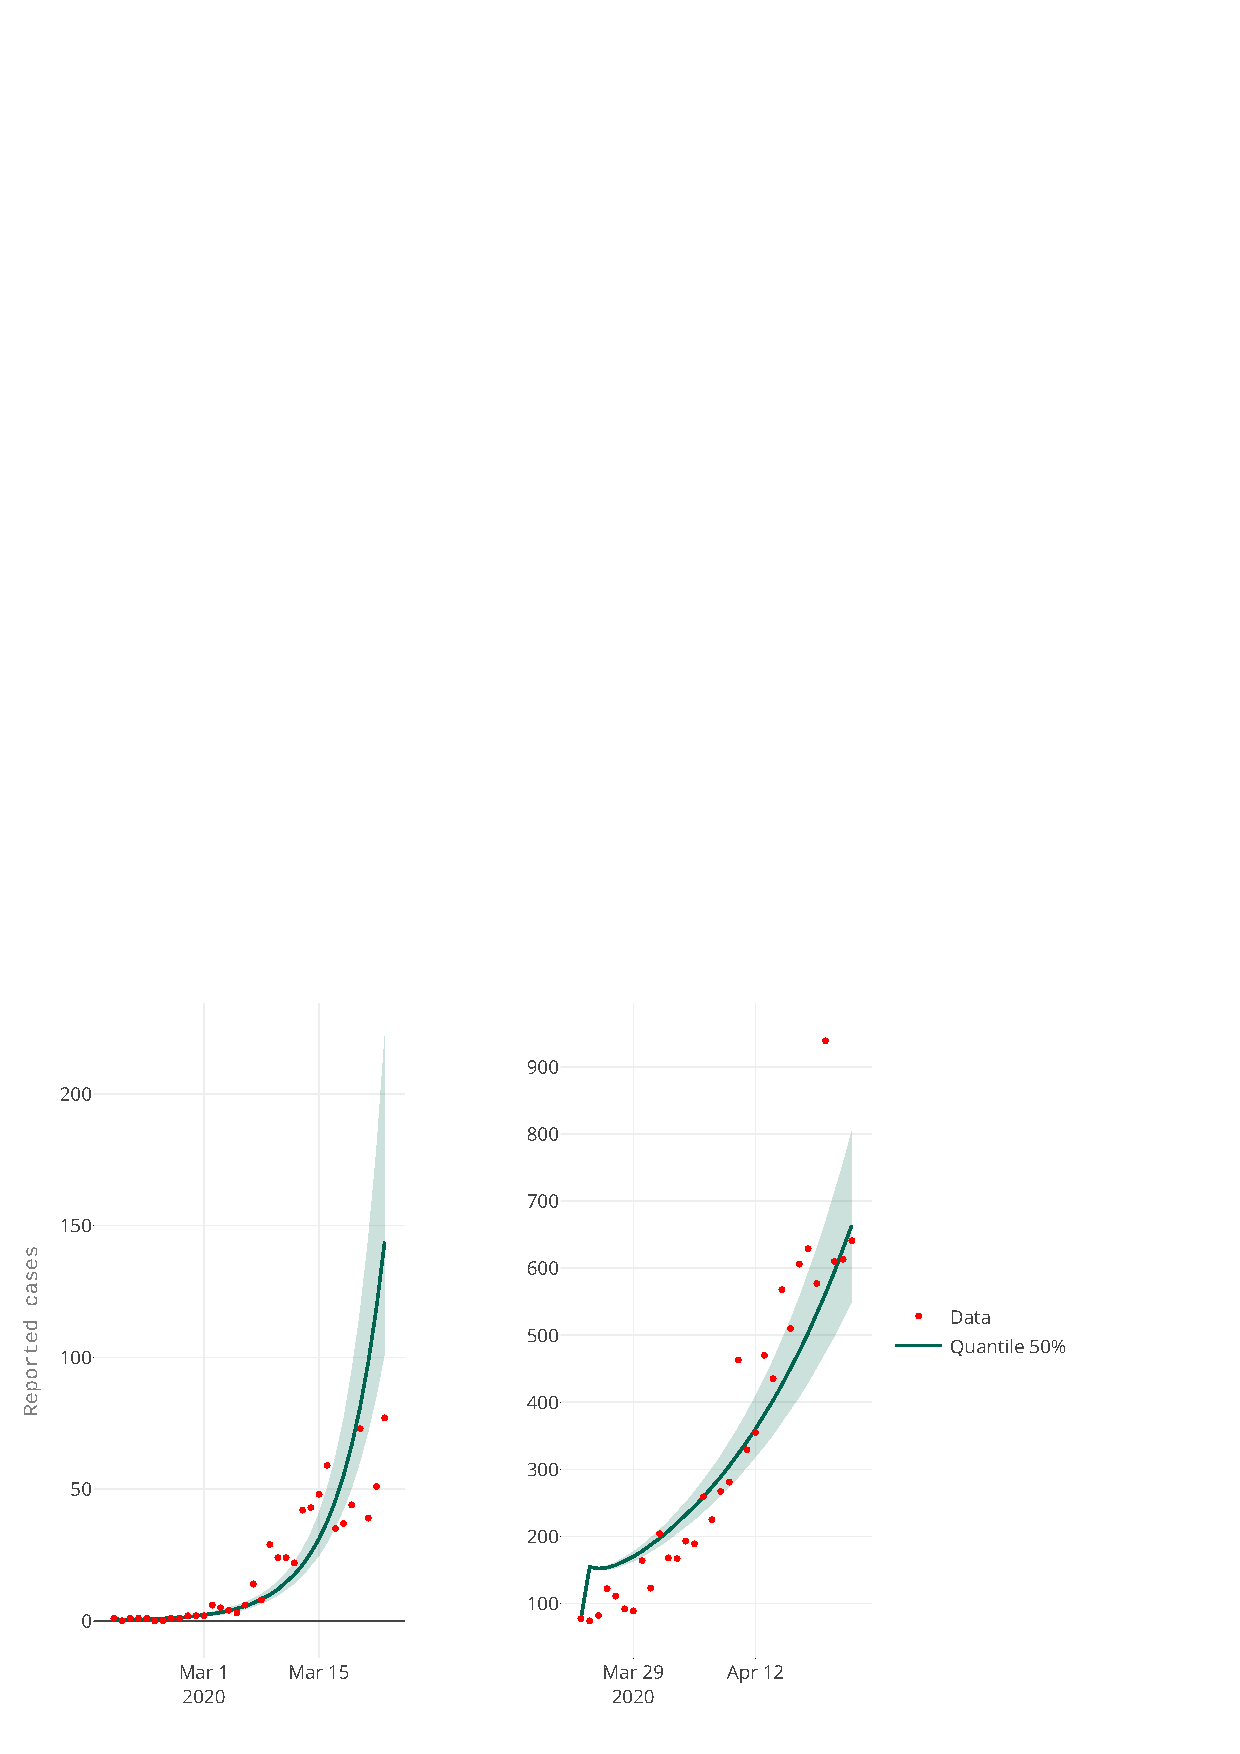
\includegraphics[width=\textwidth]{FittingCurves.png}
    \caption{Fitting curves for the early
    phase of the COVID-19 outbreak in Mexico
    City plus Mexico state. Panel A shows the
    outbreak from February 19 to March 23,
    2020, while panel B illustrates the
    outbreak from March 23 to April 23, 2020.
    Reported data are shown in blue points,
    while that solid red line represents
    quantile 50 of all solutions}
    \label{Fig:fittingcurve}
\end{figure}
%
\begin{table}[h!]
    \begin{center}
        \begin{tabular}{cc}
            \toprule
            Parameter & 95\% Confidence
            Interval
            \\
            \midrule
            $\beta_S$ & $[0.2483712,
            0.48720714]$ \\
            $\beta_A$ & $[0.1851696,
            0.32181249]$ \\
            $p$       & $[0.061, 0.2206]$ \\
            $R_0$     & $[1.702, 1.887]$\\
            \bottomrule
        \end{tabular}
        \caption{Confidence interval for some
        parameters of system~\eqref{model1},
        and for the basic reproductive number
        $(R_0)$.}\label{table_icparam4}
    \end{center}
\end{table}

On the other hand, since it is unclear when
the vaccines will be available, then we
assume that our scenarios start on the growth
stage of a second outbreak (see
\Cref{Fig:initial_conditions}) with the
objective of...
\begin{figure}[!h]
    \includegraphics[width=\textwidth]{Is_dynamics.png}
    \caption{Dynamics of the symptomatic
    individuals. Black arrow indicates the
    outbreak stage in which we start our
    simulations.}
    \label{Fig:initial_conditions}
\end{figure}


%\pagebreak
